% Options for packages loaded elsewhere
\PassOptionsToPackage{unicode}{hyperref}
\PassOptionsToPackage{hyphens}{url}
\PassOptionsToPackage{dvipsnames,svgnames,x11names}{xcolor}
%
\documentclass[
]{article}

\usepackage{amsmath,amssymb}
\usepackage{iftex}
\ifPDFTeX
  \usepackage[T1]{fontenc}
  \usepackage[utf8]{inputenc}
  \usepackage{textcomp} % provide euro and other symbols
\else % if luatex or xetex
  \usepackage{unicode-math}
  \defaultfontfeatures{Scale=MatchLowercase}
  \defaultfontfeatures[\rmfamily]{Ligatures=TeX,Scale=1}
\fi
\usepackage{lmodern}
\ifPDFTeX\else  
    % xetex/luatex font selection
    \setmainfont[]{TeX Gyre Pagella Math}
    \setsansfont[]{TeX Gyre Heros}
    \setmonofont[]{TeX Gyre Termes}
\fi
% Use upquote if available, for straight quotes in verbatim environments
\IfFileExists{upquote.sty}{\usepackage{upquote}}{}
\IfFileExists{microtype.sty}{% use microtype if available
  \usepackage[]{microtype}
  \UseMicrotypeSet[protrusion]{basicmath} % disable protrusion for tt fonts
}{}
\makeatletter
\@ifundefined{KOMAClassName}{% if non-KOMA class
  \IfFileExists{parskip.sty}{%
    \usepackage{parskip}
  }{% else
    \setlength{\parindent}{0pt}
    \setlength{\parskip}{6pt plus 2pt minus 1pt}}
}{% if KOMA class
  \KOMAoptions{parskip=half}}
\makeatother
\usepackage{xcolor}
\setlength{\emergencystretch}{3em} % prevent overfull lines
\setcounter{secnumdepth}{-\maxdimen} % remove section numbering
% Make \paragraph and \subparagraph free-standing
\makeatletter
\ifx\paragraph\undefined\else
  \let\oldparagraph\paragraph
  \renewcommand{\paragraph}{
    \@ifstar
      \xxxParagraphStar
      \xxxParagraphNoStar
  }
  \newcommand{\xxxParagraphStar}[1]{\oldparagraph*{#1}\mbox{}}
  \newcommand{\xxxParagraphNoStar}[1]{\oldparagraph{#1}\mbox{}}
\fi
\ifx\subparagraph\undefined\else
  \let\oldsubparagraph\subparagraph
  \renewcommand{\subparagraph}{
    \@ifstar
      \xxxSubParagraphStar
      \xxxSubParagraphNoStar
  }
  \newcommand{\xxxSubParagraphStar}[1]{\oldsubparagraph*{#1}\mbox{}}
  \newcommand{\xxxSubParagraphNoStar}[1]{\oldsubparagraph{#1}\mbox{}}
\fi
\makeatother

\usepackage{color}
\usepackage{fancyvrb}
\newcommand{\VerbBar}{|}
\newcommand{\VERB}{\Verb[commandchars=\\\{\}]}
\DefineVerbatimEnvironment{Highlighting}{Verbatim}{commandchars=\\\{\}}
% Add ',fontsize=\small' for more characters per line
\usepackage{framed}
\definecolor{shadecolor}{RGB}{241,243,245}
\newenvironment{Shaded}{\begin{snugshade}}{\end{snugshade}}
\newcommand{\AlertTok}[1]{\textcolor[rgb]{0.68,0.00,0.00}{#1}}
\newcommand{\AnnotationTok}[1]{\textcolor[rgb]{0.37,0.37,0.37}{#1}}
\newcommand{\AttributeTok}[1]{\textcolor[rgb]{0.40,0.45,0.13}{#1}}
\newcommand{\BaseNTok}[1]{\textcolor[rgb]{0.68,0.00,0.00}{#1}}
\newcommand{\BuiltInTok}[1]{\textcolor[rgb]{0.00,0.23,0.31}{#1}}
\newcommand{\CharTok}[1]{\textcolor[rgb]{0.13,0.47,0.30}{#1}}
\newcommand{\CommentTok}[1]{\textcolor[rgb]{0.37,0.37,0.37}{#1}}
\newcommand{\CommentVarTok}[1]{\textcolor[rgb]{0.37,0.37,0.37}{\textit{#1}}}
\newcommand{\ConstantTok}[1]{\textcolor[rgb]{0.56,0.35,0.01}{#1}}
\newcommand{\ControlFlowTok}[1]{\textcolor[rgb]{0.00,0.23,0.31}{\textbf{#1}}}
\newcommand{\DataTypeTok}[1]{\textcolor[rgb]{0.68,0.00,0.00}{#1}}
\newcommand{\DecValTok}[1]{\textcolor[rgb]{0.68,0.00,0.00}{#1}}
\newcommand{\DocumentationTok}[1]{\textcolor[rgb]{0.37,0.37,0.37}{\textit{#1}}}
\newcommand{\ErrorTok}[1]{\textcolor[rgb]{0.68,0.00,0.00}{#1}}
\newcommand{\ExtensionTok}[1]{\textcolor[rgb]{0.00,0.23,0.31}{#1}}
\newcommand{\FloatTok}[1]{\textcolor[rgb]{0.68,0.00,0.00}{#1}}
\newcommand{\FunctionTok}[1]{\textcolor[rgb]{0.28,0.35,0.67}{#1}}
\newcommand{\ImportTok}[1]{\textcolor[rgb]{0.00,0.46,0.62}{#1}}
\newcommand{\InformationTok}[1]{\textcolor[rgb]{0.37,0.37,0.37}{#1}}
\newcommand{\KeywordTok}[1]{\textcolor[rgb]{0.00,0.23,0.31}{\textbf{#1}}}
\newcommand{\NormalTok}[1]{\textcolor[rgb]{0.00,0.23,0.31}{#1}}
\newcommand{\OperatorTok}[1]{\textcolor[rgb]{0.37,0.37,0.37}{#1}}
\newcommand{\OtherTok}[1]{\textcolor[rgb]{0.00,0.23,0.31}{#1}}
\newcommand{\PreprocessorTok}[1]{\textcolor[rgb]{0.68,0.00,0.00}{#1}}
\newcommand{\RegionMarkerTok}[1]{\textcolor[rgb]{0.00,0.23,0.31}{#1}}
\newcommand{\SpecialCharTok}[1]{\textcolor[rgb]{0.37,0.37,0.37}{#1}}
\newcommand{\SpecialStringTok}[1]{\textcolor[rgb]{0.13,0.47,0.30}{#1}}
\newcommand{\StringTok}[1]{\textcolor[rgb]{0.13,0.47,0.30}{#1}}
\newcommand{\VariableTok}[1]{\textcolor[rgb]{0.07,0.07,0.07}{#1}}
\newcommand{\VerbatimStringTok}[1]{\textcolor[rgb]{0.13,0.47,0.30}{#1}}
\newcommand{\WarningTok}[1]{\textcolor[rgb]{0.37,0.37,0.37}{\textit{#1}}}

\providecommand{\tightlist}{%
  \setlength{\itemsep}{0pt}\setlength{\parskip}{0pt}}\usepackage{longtable,booktabs,array}
\usepackage{calc} % for calculating minipage widths
% Correct order of tables after \paragraph or \subparagraph
\usepackage{etoolbox}
\makeatletter
\patchcmd\longtable{\par}{\if@noskipsec\mbox{}\fi\par}{}{}
\makeatother
% Allow footnotes in longtable head/foot
\IfFileExists{footnotehyper.sty}{\usepackage{footnotehyper}}{\usepackage{footnote}}
\makesavenoteenv{longtable}
\usepackage{graphicx}
\makeatletter
\newsavebox\pandoc@box
\newcommand*\pandocbounded[1]{% scales image to fit in text height/width
  \sbox\pandoc@box{#1}%
  \Gscale@div\@tempa{\textheight}{\dimexpr\ht\pandoc@box+\dp\pandoc@box\relax}%
  \Gscale@div\@tempb{\linewidth}{\wd\pandoc@box}%
  \ifdim\@tempb\p@<\@tempa\p@\let\@tempa\@tempb\fi% select the smaller of both
  \ifdim\@tempa\p@<\p@\scalebox{\@tempa}{\usebox\pandoc@box}%
  \else\usebox{\pandoc@box}%
  \fi%
}
% Set default figure placement to htbp
\def\fps@figure{htbp}
\makeatother
% definitions for citeproc citations
\NewDocumentCommand\citeproctext{}{}
\NewDocumentCommand\citeproc{mm}{%
  \begingroup\def\citeproctext{#2}\cite{#1}\endgroup}
\makeatletter
 % allow citations to break across lines
 \let\@cite@ofmt\@firstofone
 % avoid brackets around text for \cite:
 \def\@biblabel#1{}
 \def\@cite#1#2{{#1\if@tempswa , #2\fi}}
\makeatother
\newlength{\cslhangindent}
\setlength{\cslhangindent}{1.5em}
\newlength{\csllabelwidth}
\setlength{\csllabelwidth}{3em}
\newenvironment{CSLReferences}[2] % #1 hanging-indent, #2 entry-spacing
 {\begin{list}{}{%
  \setlength{\itemindent}{0pt}
  \setlength{\leftmargin}{0pt}
  \setlength{\parsep}{0pt}
  % turn on hanging indent if param 1 is 1
  \ifodd #1
   \setlength{\leftmargin}{\cslhangindent}
   \setlength{\itemindent}{-1\cslhangindent}
  \fi
  % set entry spacing
  \setlength{\itemsep}{#2\baselineskip}}}
 {\end{list}}
\usepackage{calc}
\newcommand{\CSLBlock}[1]{\hfill\break\parbox[t]{\linewidth}{\strut\ignorespaces#1\strut}}
\newcommand{\CSLLeftMargin}[1]{\parbox[t]{\csllabelwidth}{\strut#1\strut}}
\newcommand{\CSLRightInline}[1]{\parbox[t]{\linewidth - \csllabelwidth}{\strut#1\strut}}
\newcommand{\CSLIndent}[1]{\hspace{\cslhangindent}#1}

\makeatletter
\@ifpackageloaded{caption}{}{\usepackage{caption}}
\AtBeginDocument{%
\ifdefined\contentsname
  \renewcommand*\contentsname{Table of contents}
\else
  \newcommand\contentsname{Table of contents}
\fi
\ifdefined\listfigurename
  \renewcommand*\listfigurename{List of Figures}
\else
  \newcommand\listfigurename{List of Figures}
\fi
\ifdefined\listtablename
  \renewcommand*\listtablename{List of Tables}
\else
  \newcommand\listtablename{List of Tables}
\fi
\ifdefined\figurename
  \renewcommand*\figurename{Figure}
\else
  \newcommand\figurename{Figure}
\fi
\ifdefined\tablename
  \renewcommand*\tablename{Table}
\else
  \newcommand\tablename{Table}
\fi
}
\@ifpackageloaded{float}{}{\usepackage{float}}
\floatstyle{ruled}
\@ifundefined{c@chapter}{\newfloat{codelisting}{h}{lop}}{\newfloat{codelisting}{h}{lop}[chapter]}
\floatname{codelisting}{Listing}
\newcommand*\listoflistings{\listof{codelisting}{List of Listings}}
\makeatother
\makeatletter
\makeatother
\makeatletter
\@ifpackageloaded{caption}{}{\usepackage{caption}}
\@ifpackageloaded{subcaption}{}{\usepackage{subcaption}}
\makeatother

\ifLuaTeX
\usepackage[bidi=basic]{babel}
\else
\usepackage[bidi=default]{babel}
\fi
\babelprovide[main,import]{canadian}
\ifPDFTeX
\else
\babelfont{rm}[]{TeX Gyre Pagella Math}
\fi
% get rid of language-specific shorthands (see #6817):
\let\LanguageShortHands\languageshorthands
\def\languageshorthands#1{}
\ifLuaTeX
  \usepackage[english]{selnolig} % disable illegal ligatures
\fi
\usepackage{bookmark}

\IfFileExists{xurl.sty}{\usepackage{xurl}}{} % add URL line breaks if available
\urlstyle{same} % disable monospaced font for URLs
\hypersetup{
  pdftitle={A Julia toolkit for species distribution data},
  pdflang={en-CA},
  colorlinks=true,
  linkcolor={blue},
  filecolor={Maroon},
  citecolor={Blue},
  urlcolor={Blue},
  pdfcreator={LaTeX via pandoc}}



\title{A Julia toolkit for species distribution data}
\author{Timothée Poisot %
%
\textsuperscript{%
%
1%
}%
}
\date{}

\usepackage{setspace}
\usepackage[left,pagewise]{lineno}
\usepackage[letterpaper]{geometry}

\singlespacing
\geometry{lmargin=3cm}
\geometry{rmargin=5cm}

\begin{document}


{\bfseries\sffamily\Large A Julia toolkit for species distribution data}
\vskip 1em
Timothée Poisot %
%
\textsuperscript{%
%
1%
}%

\vskip 2em
{\small
\textbf{Abstract:} LATER
\vskip 1em
}
\vskip 4em
\flushleft


\section{Introduction}\label{introduction}

Species Distribution Models (SDMs) are one of the most effective
predictive approach to study the global distribution of biodiversity
(Elith \& Leathwick, 2009). The training and evaluation of a SDM
requires many steps, governing both its design and reporting (Zurell et
al., 2020) and ultimate use and interpretation (Araújo et al., 2019). In
the recent years, there has been an increase in the number of software
packages and tools to assist ecologists with the development of species
distribution models. As Kass et al. (2024) point out, this increase in
the diversity of packages (most of them in the \textbf{R} language) is a
good thing, as it can accommodate multiple workflows, and contributes to
the adoption of good practices in the field.

Because the practice of species distribution modeling and analysis
usually involve many different data types, tools that can provide an
integrated environment are important: many existing packages have been
designed independently, and therefore may suffer when it comes to
interoperability. In this manuscript, we present
\textbf{SpeciesDistributionToolkit} (abbreviated as \textbf{SDT}), a
meta-package for the \textbf{Julia} programming language, offering an
integrated environment for the retrieval, formatting, and interpretation
of data relevant to the modeling of species distributions.

Griffith et al. (2024) for large-scale SDM

\section{Application description}\label{application-description}

\ldots{}

\subsection{Component packages}\label{component-packages}

An overview of the \textbf{SDT} package is given in
Figure~\ref{fig-components}. The project is organized as a ``monorepo'',
in which multiple packages live. This allows expanding the scope of the
package by moving functionalities into new component packages, without
complexifying the installation process. At \textbf{SDT} is registered in
the \textbf{Julia} package repository, it can be installed with:

\begin{Shaded}
\begin{Highlighting}[]
\ImportTok{import} \BuiltInTok{Pkg;}\NormalTok{ Pkg.add("SpeciesDistributionToolkit")}
\end{Highlighting}
\end{Shaded}

When loading the \textbf{SDT} package with
\texttt{using\ SpeciesDistributionToolkit}, all component packages are
automatically and transparently loaded. Therefore, users do not need to
know where a specific method or function resides to use it. In the next
section, we discuss how this modular design ensure that we can grow the
functionality of the toolkit over time, while maintaining strict
backward compatibility \emph{and} allowing full reproducibility of an
analysis.

\begin{figure}

\centering{

\pandocbounded{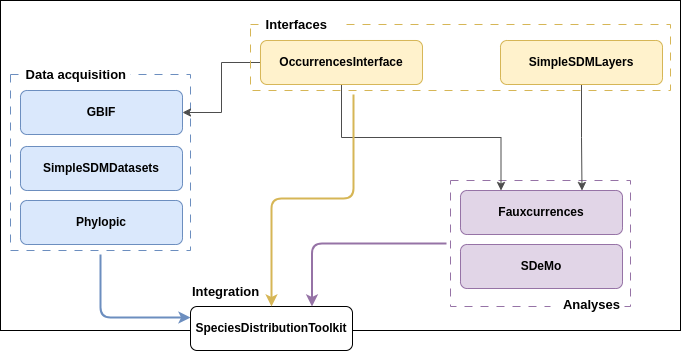
\includegraphics[keepaspectratio]{figures/SDT.png}}

}

\caption{\label{fig-components}Overview of the packages}

\end{figure}%

\textbf{GBIF}

\textbf{SimpleSDMDatasets}

\textbf{Phylopic}

\textbf{OccurrencesInterface}

\textbf{SimpleSDMLayers}

The \textbf{Fauxcurrences} packages is inspired by the work of Osborne
et al. (2022), and

\textbf{SDeMo}

\subsection{Software information}\label{software-information}

\textbf{SDT} uses the built-in \textbf{Julia} package manager to ensure
that the version of all dependencies are kept up to date. Furthermore,
we use strict semantic versioning: major versions correspond to no
breaking changes in user-developped code, minor versions increase with
additional functionalities, and patch releases cover minor bug fixes or
documentation changes. All packages have a \emph{CHANGELOG} file, which
documents what changes are included in each release.

This strict reliance on semantic versioning solves the issues of
maintaining compatibility when new functionalities are added: all
releases in the \emph{v1.x.x} branch of \textbf{SDT} depend on component
packages in their respective \emph{v1.x.x} branch, and users can benefit
from now functionalities without risking to break existing code. This
behavior is extensively tested, both using unit tests, and through
integration testing generated as part of the online documentation.

Kellner et al. (2025) reported that about 20\% of failures to reproduce
species distribution or abundance modeling code was related to package
issues. The strict reliance on semantic versioning, alongside technical
choices in the \textbf{Julia} package manager and repository, means that
it is possible to specify the full version of all dependencies used in a
project, which addresses this important obstacle to reproducibility.

\subsection{Integration with other
packages}\label{integration-with-other-packages}

The \textbf{SDT} package benefits from close integration with other
packages in the Julia universe. Notably, this includes \textbf{Makie}
(and all related backends) for plotting and data visualisation, where
usual plot types are overloaded for layer and occurrence data. Most data
can be exported using the \textbf{Tables} interface, which allows data
to be consumed by other packages like \textbf{DataFrames} and
\textbf{MLJ}. Interfaces internal to Julia are also implemented whenever
they make sense. Layers behave like arrays, are iterable, and
broadcastable; occurrences collections are arrays and iterables. Beyong
supporting external interfaces, \textbf{SDT} defines its own internally.
Access to raster data is supported by a trait-based interface for
\textbf{SimpleSDMDatasets}, and one of the component packages
(\textbf{OccurrencesInterface} implements a minimalist interface to
facilite the consumption of occurrence data.

Internal use of other interfaces like StatsAPI

\section{Illustrative case studies}\label{illustrative-case-studies}

In this section, we provide a series of case studies, meant to
illustrate the use of the package. The on-line documentation offers
longer tutorials, as well as a series of how-to vignettes to illustrate
the full scope of what the package allows. The code for each of these
case studies is available as fully independent Jupyter notebooks,
forming the supplementary material of this article. The example we use
throughout is the distribution of \emph{Akodon montensis} (Rodentia,
family Cricetidae), and a host or orthohantaviruses (Burgos et al.,
2021; Owen et al., 2010), in Paraguay. As the notebooks accompanying
this article cover the full code required to run these examples, we do
not present code snippets in the main text, and instead focus on
explaining which component packages are used in each example.

\subsection{Landcover consensus map}\label{landcover-consensus-map}

In this case study, we retrieve the land cover data from Tuanmu \& Jetz
(2014), clip them to a GeoJSON polygon describing the country of
Paraguay (\textbf{SDT} can download data directly from
\texttt{gadm.org}), and apply the \texttt{mosaic} operation to figure
out which class is the most locally abundant. This case study uses the
\textbf{SimpleSDMDatasets} package to download (and locally cache) the
raster data, as well as the \textbf{SimpleSDMLayers} package to provide
basic utility functions on raster data.

\begin{figure}[H]

\centering{

\pandocbounded{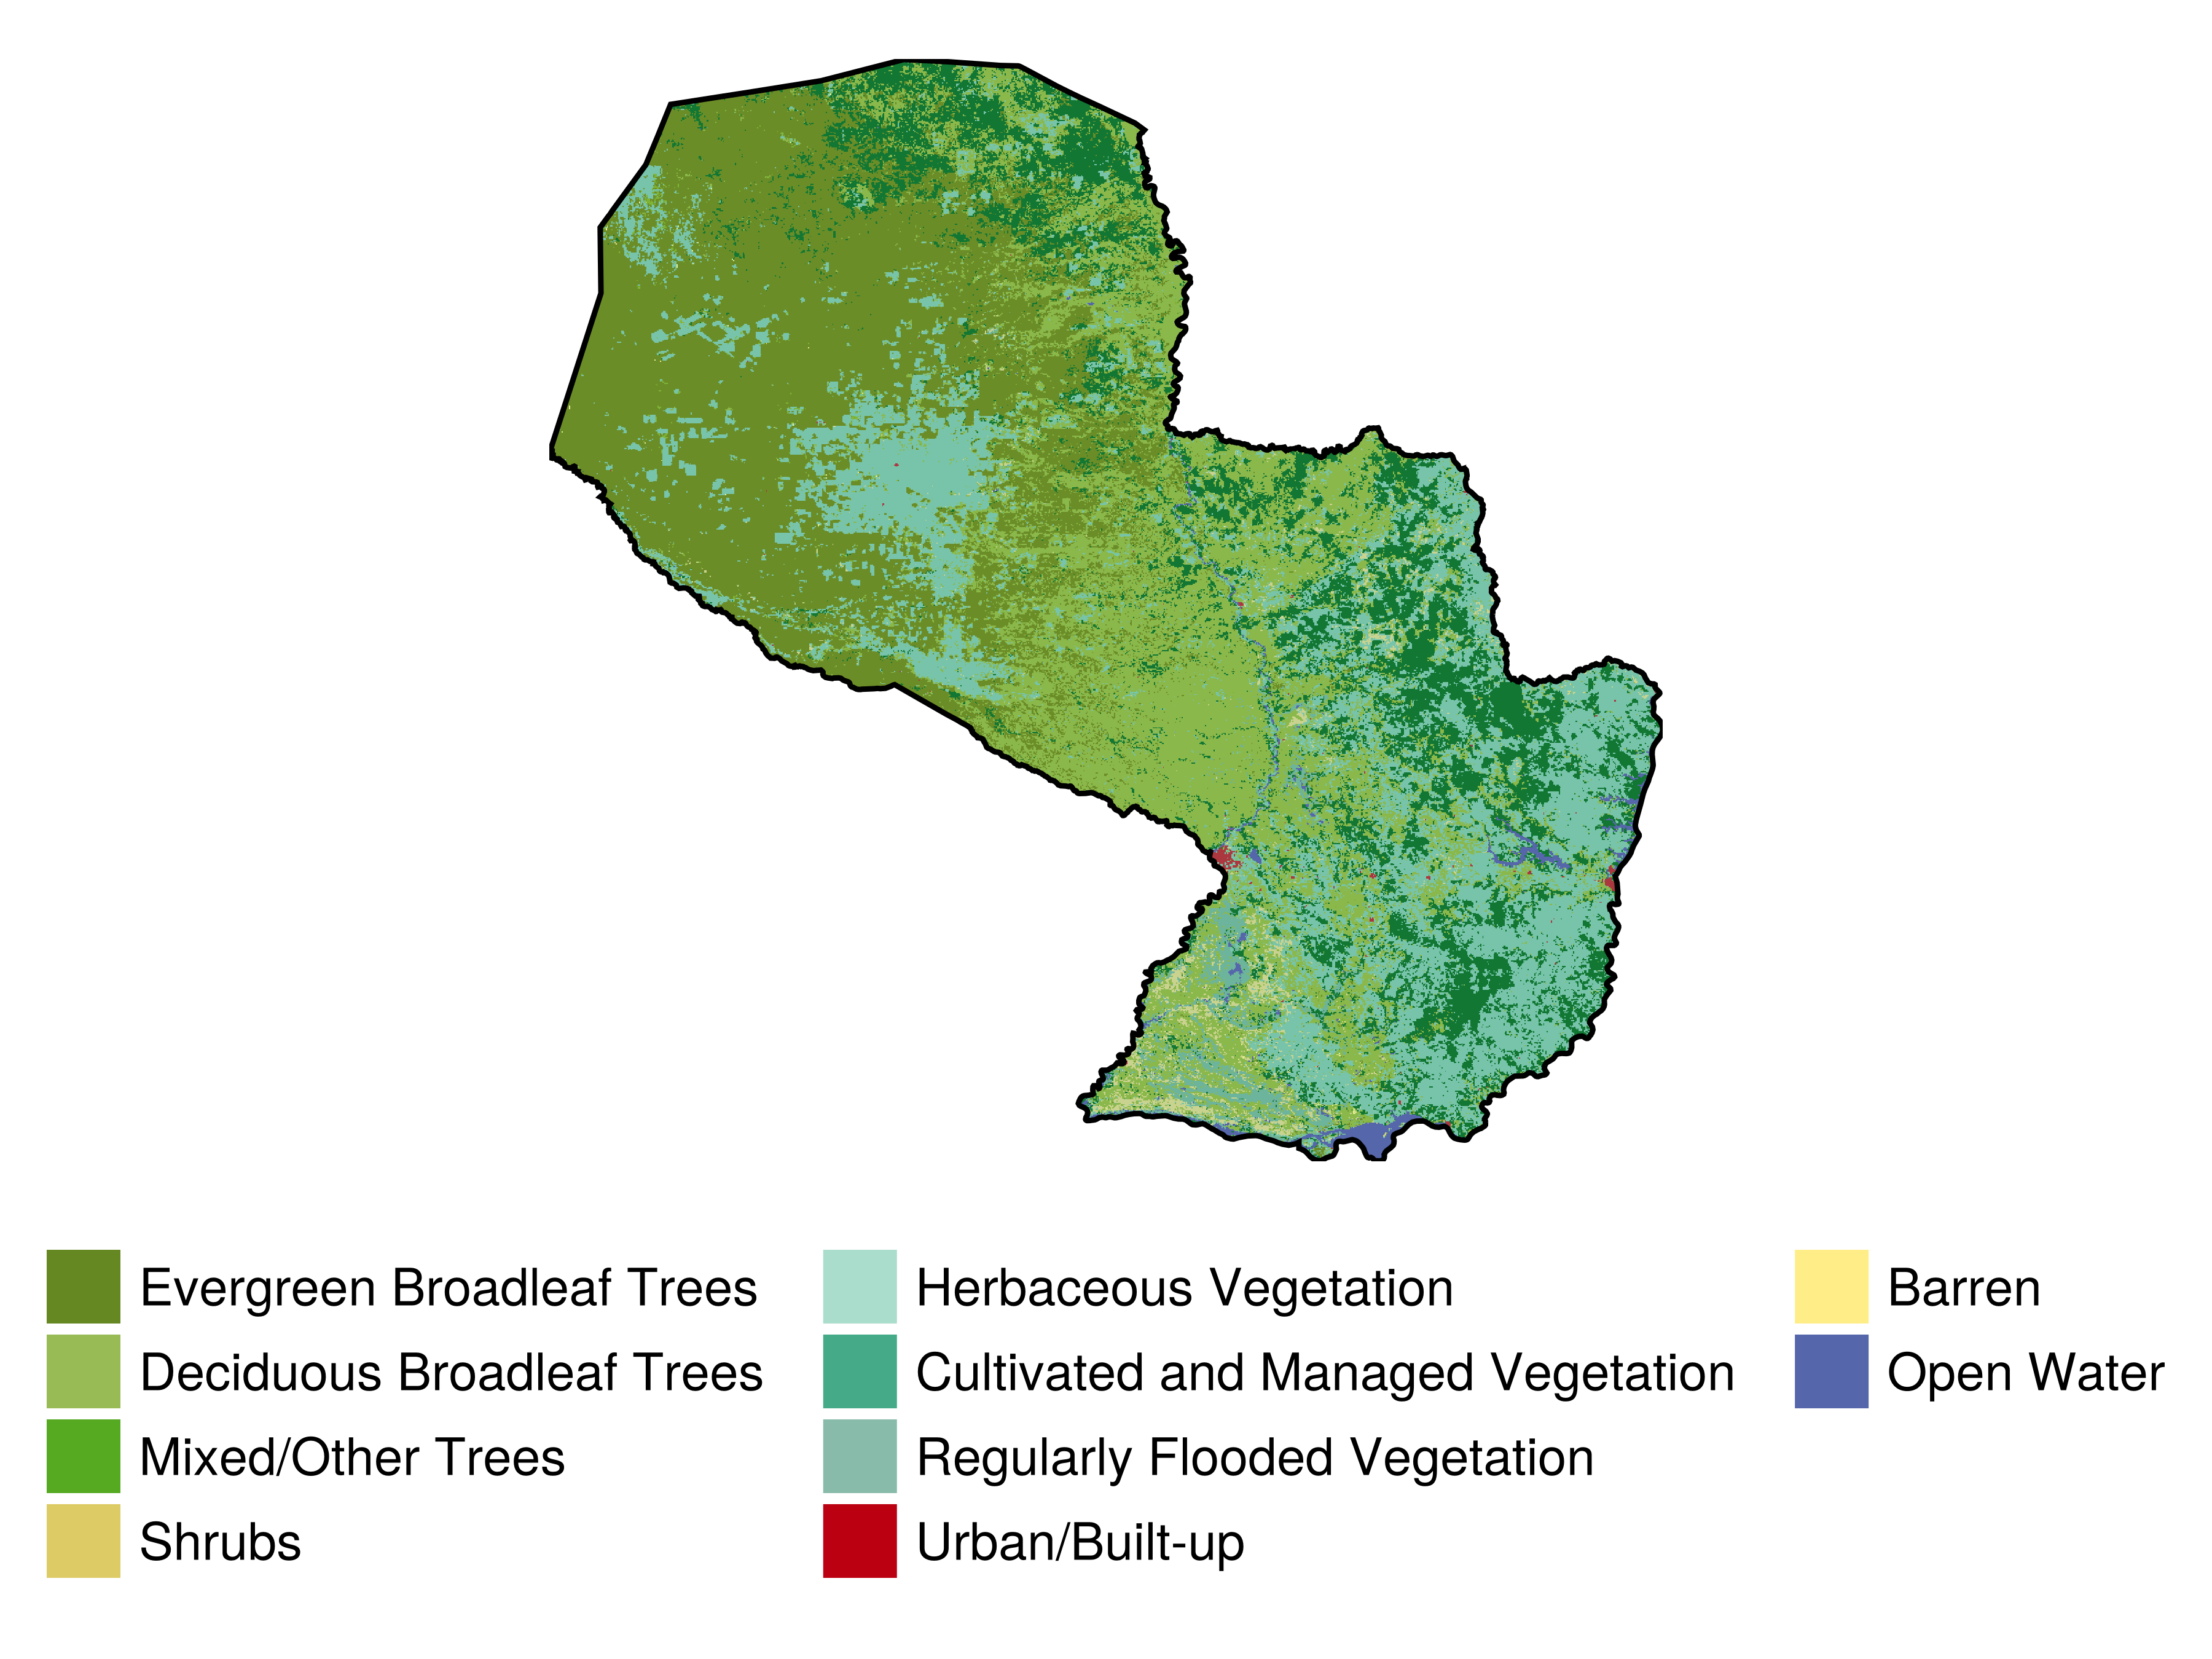
\includegraphics[keepaspectratio]{index_files/figure-latex/appendix-consensus-fig-landcover-consensus-output-1.png}}

}

\caption{\label{fig-landcover-consensus}yeah}

\end{figure}%

\subsection{Using data from GBIF}\label{using-data-from-gbif}

(GBIF: The Global Biodiversity Information Facility, 2025)

(Karger et al., 2017)

\begin{figure}[H]

\centering{

\pandocbounded{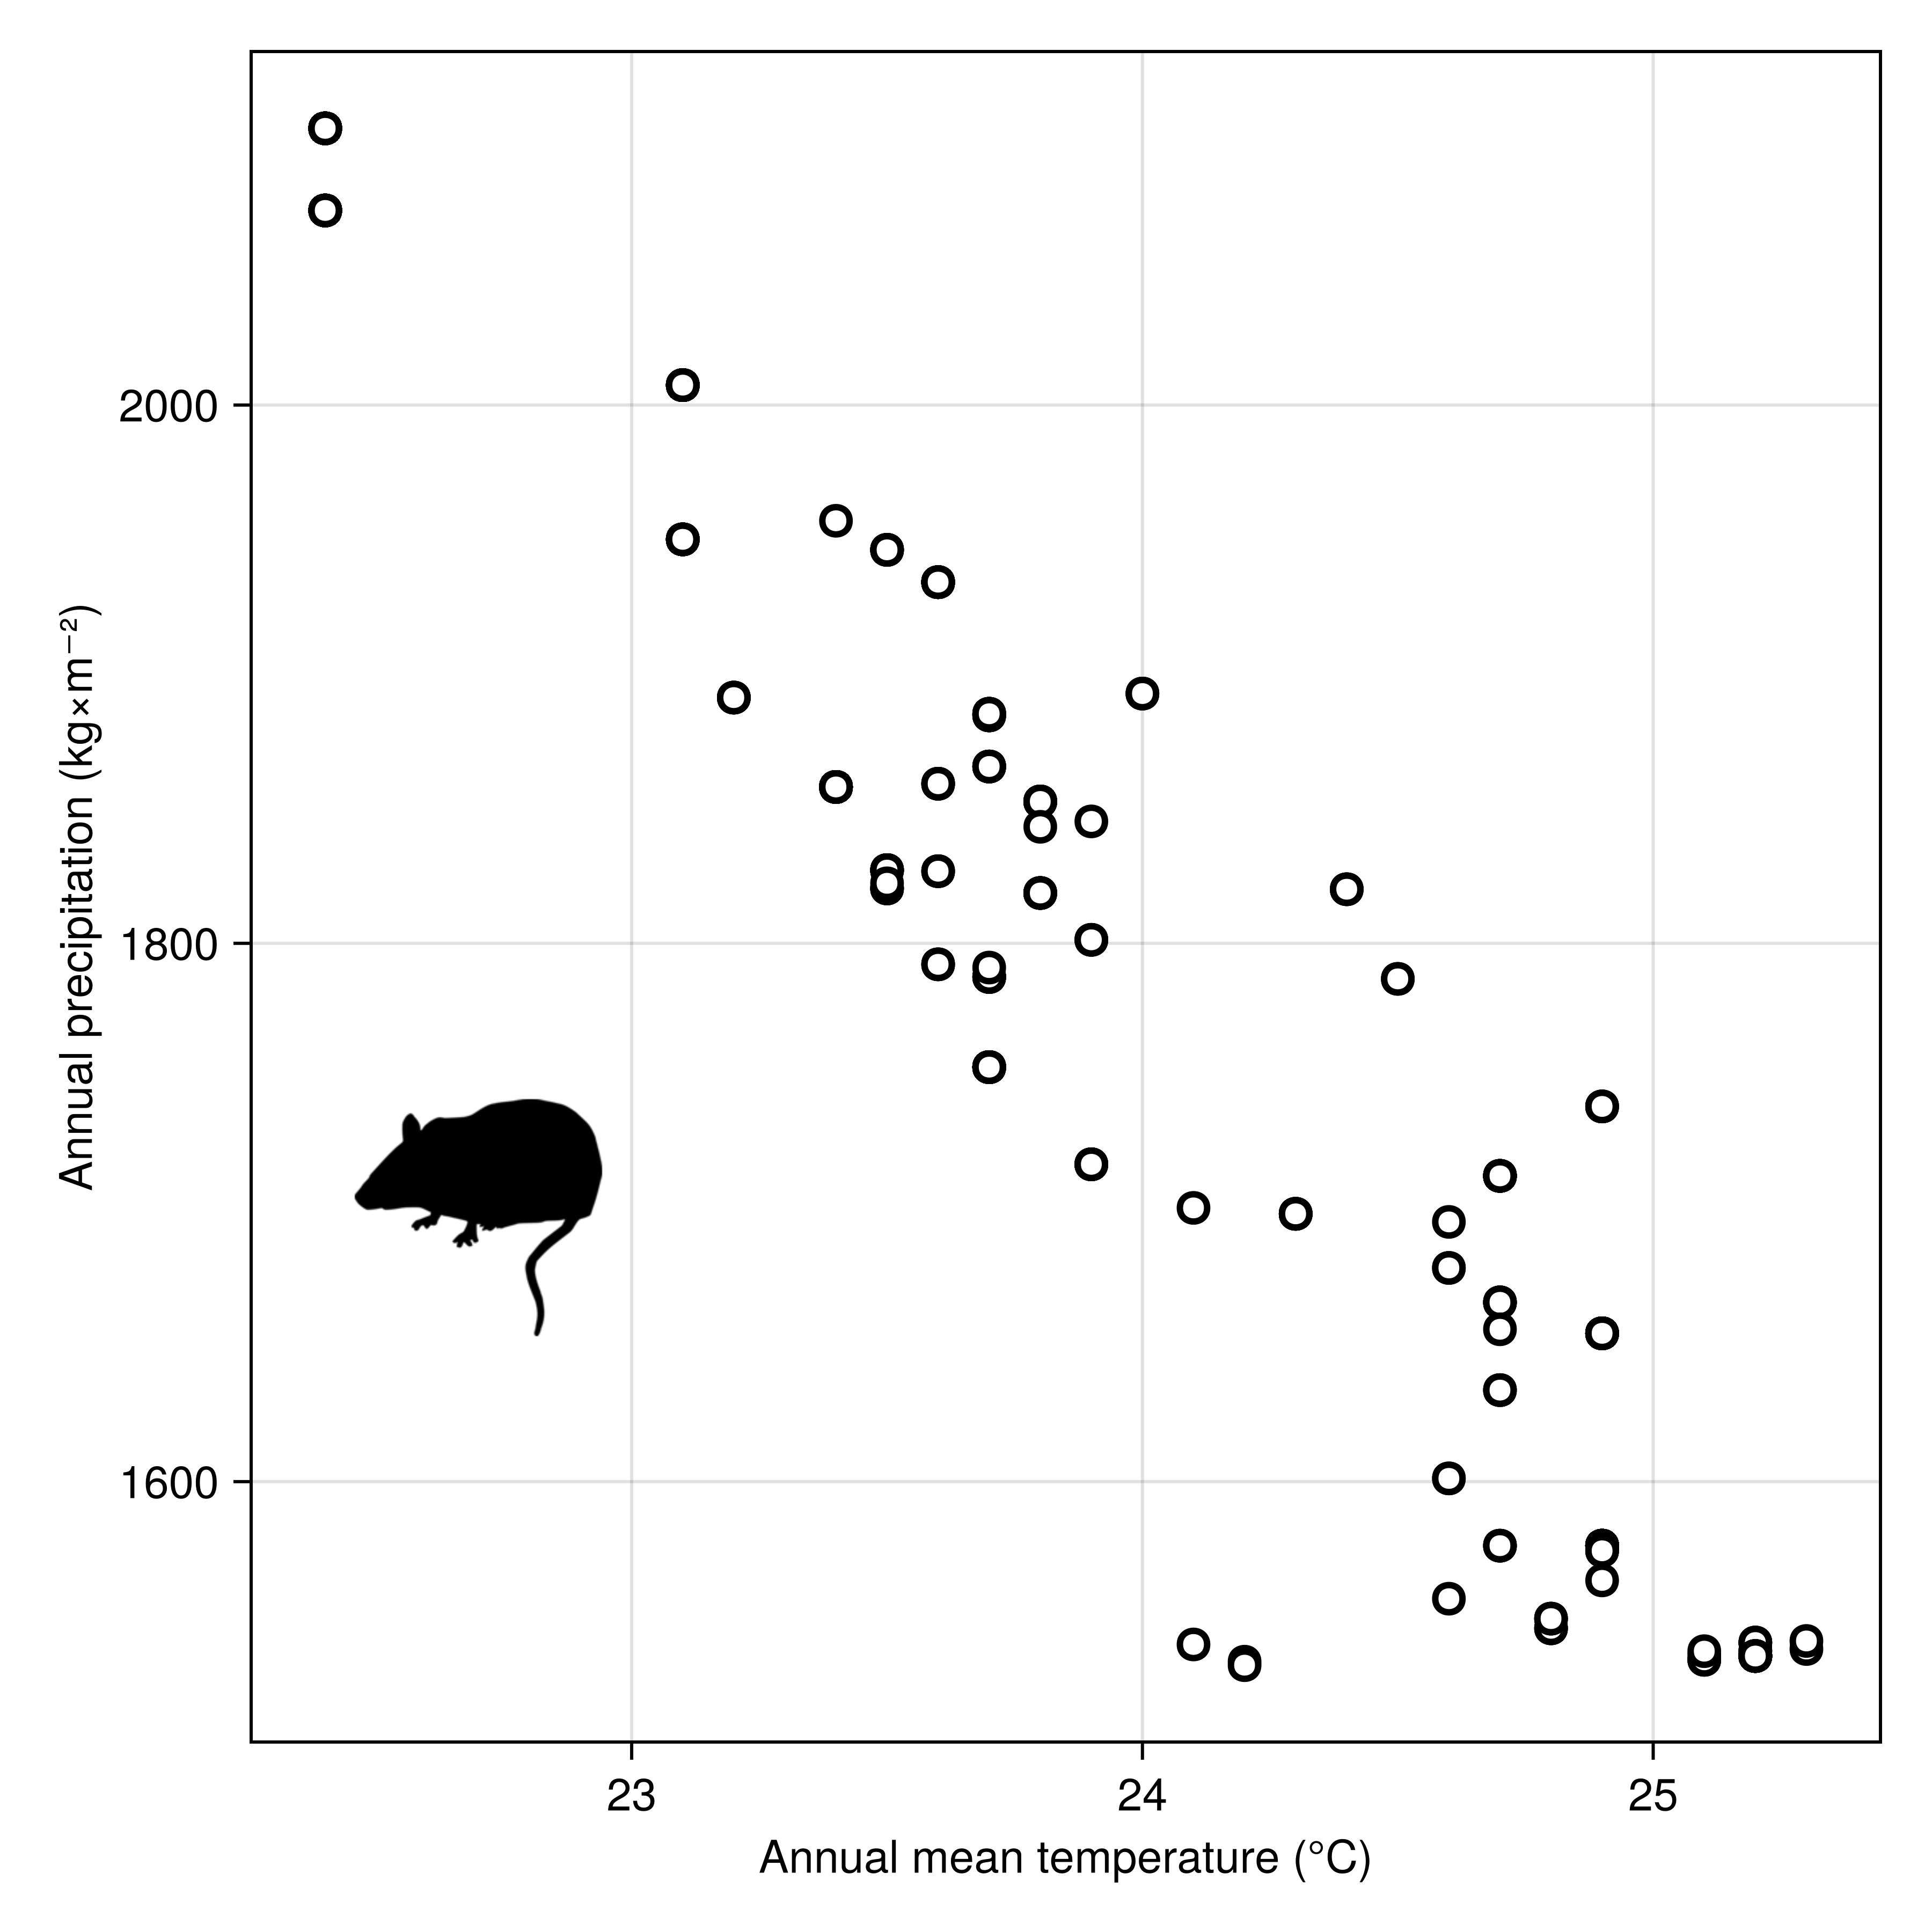
\includegraphics[keepaspectratio]{index_files/figure-latex/appendix-gbif-fig-gbif-phylopic-output-1.png}}

}

\caption{\label{fig-gbif-phylopic}yeah}

\end{figure}%

In practice, although the data are retrieved using the \textbf{GBIF}
package, they are used internally by \textbf{SDT} through the
\textbf{OccurrencesInterface} package. This package defines a small
convention to handle georeferenced occurrence data, and allows to
transparently integrate additional occurrence sources. By defining five
methods for a custom data type, users can plug-in any occurrence data
source and enjoy full compatibility with the entire \textbf{SDT}
functionalities.

\subsection{Training a species distribution
model}\label{training-a-species-distribution-model}

(Bagnall et al., 2018)

\begin{figure}[H]

\centering{

\pandocbounded{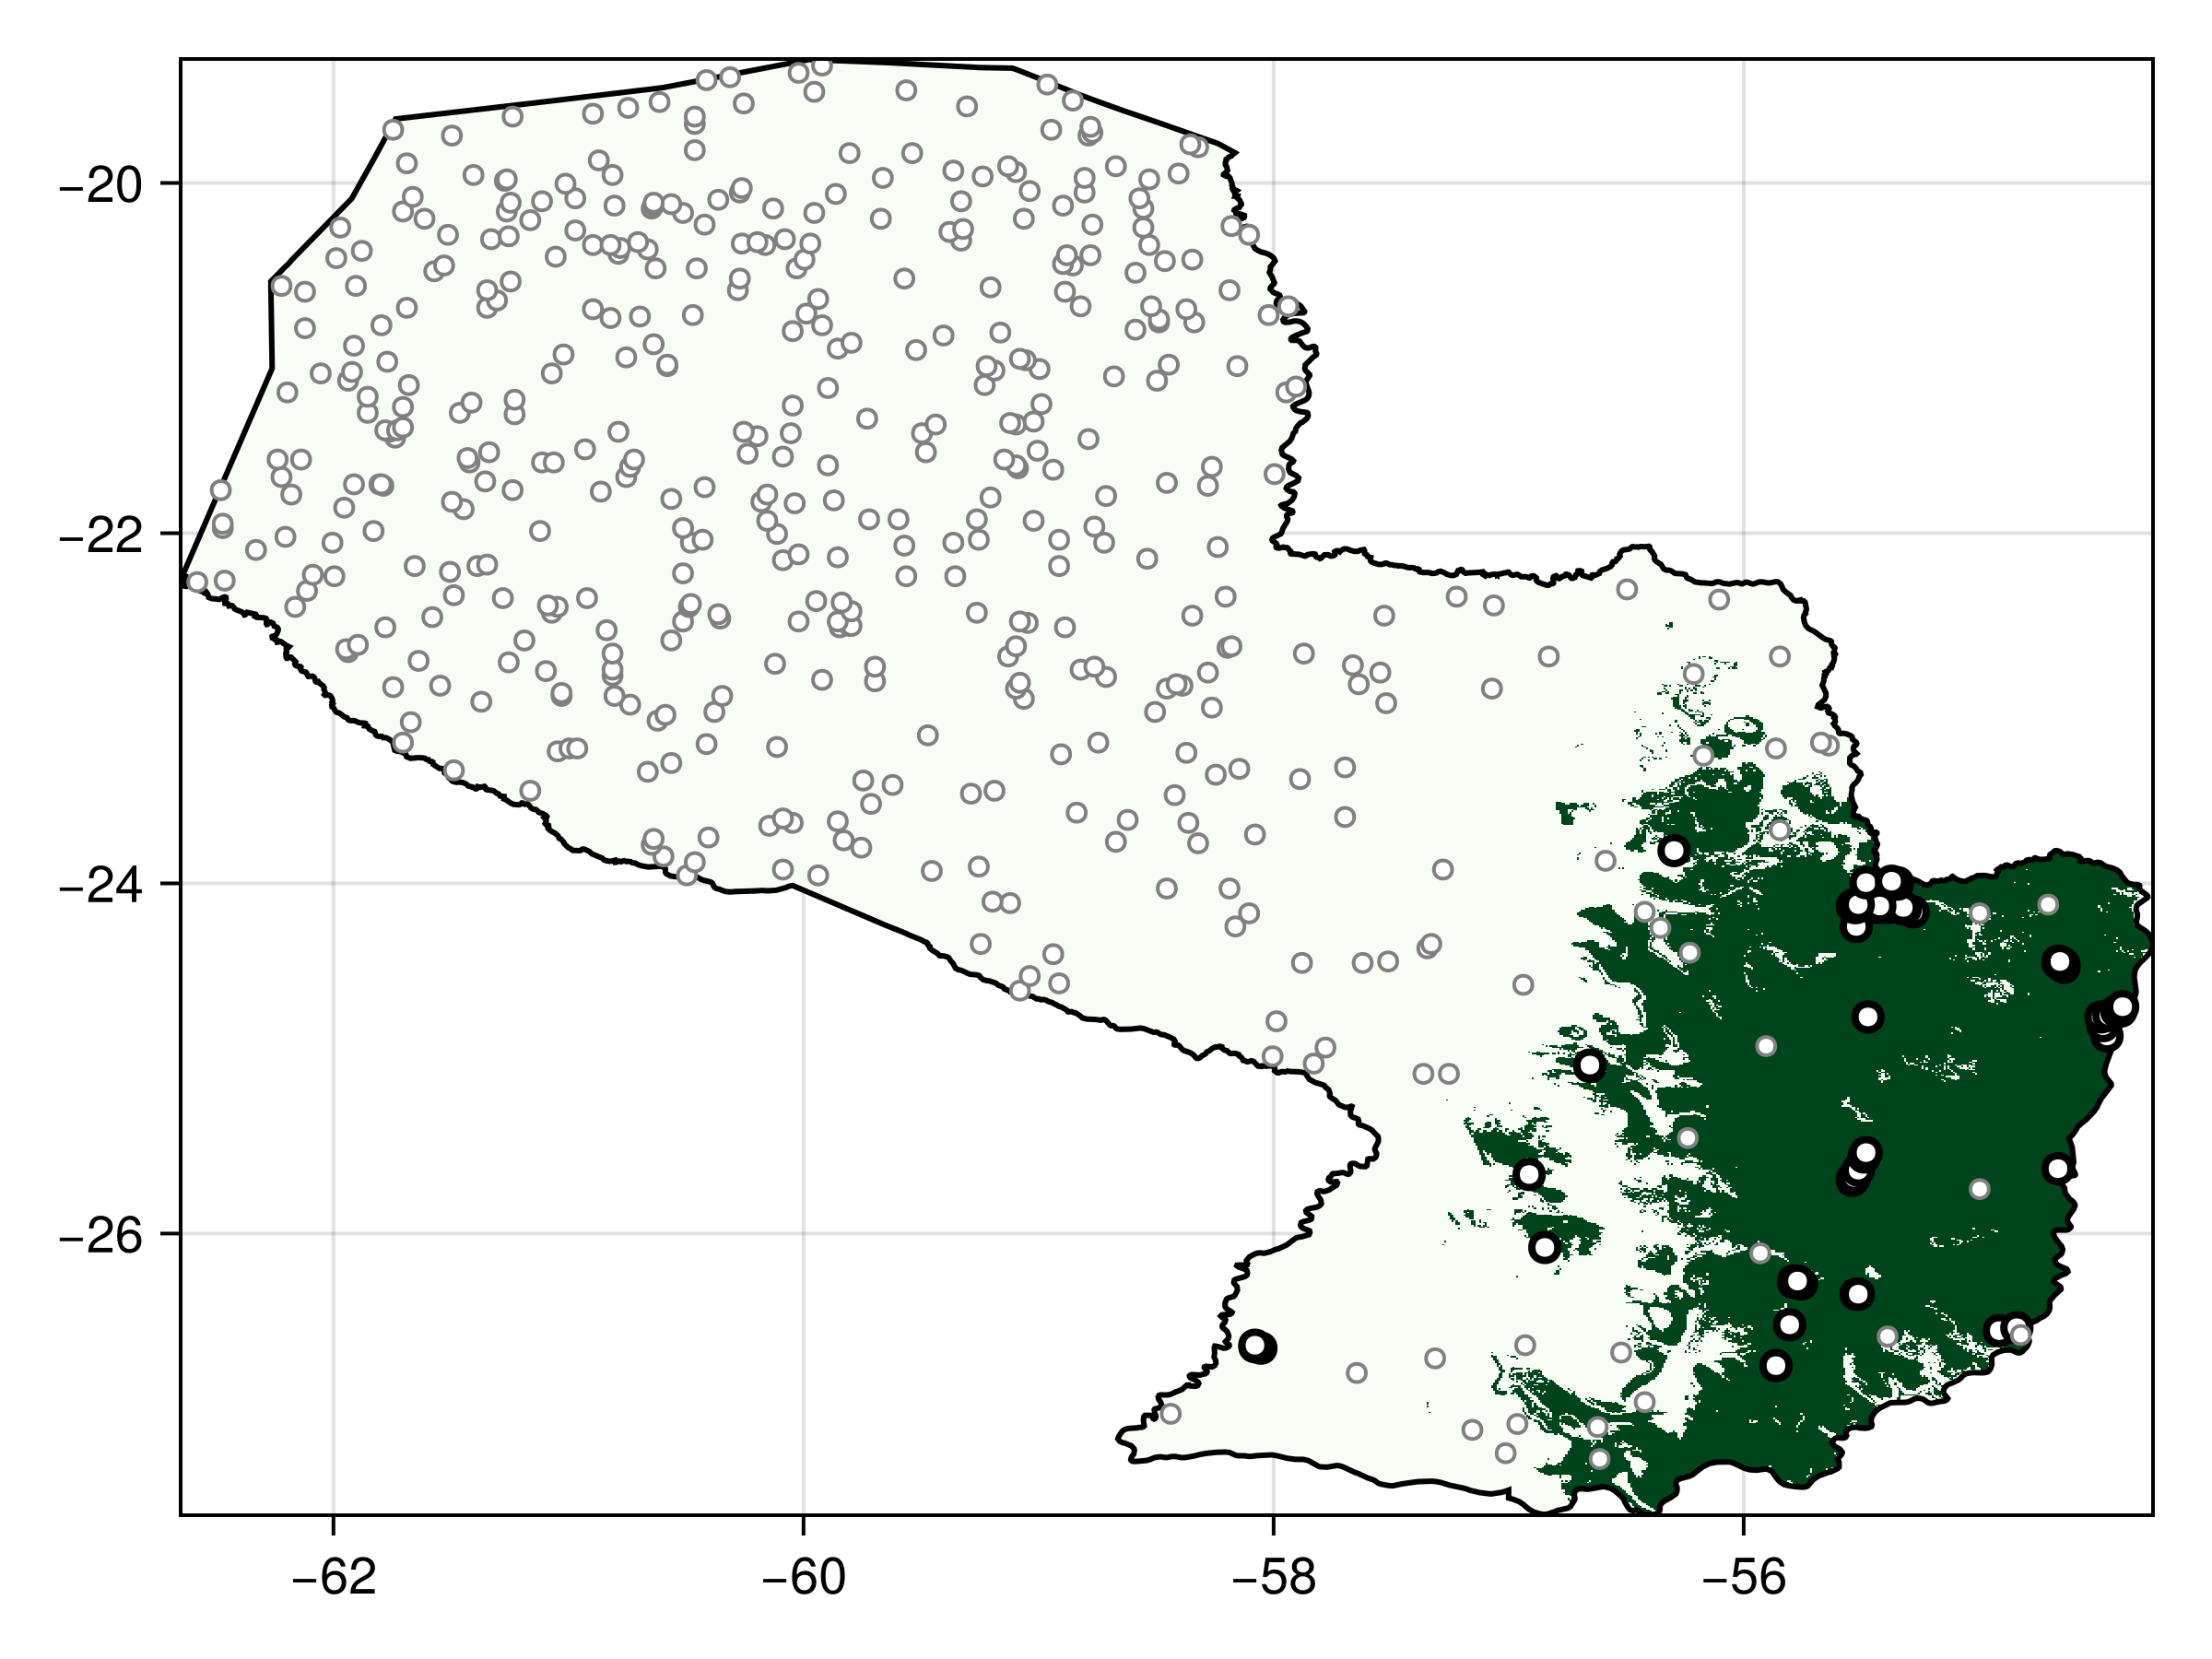
\includegraphics[keepaspectratio]{index_files/figure-latex/appendix-sdm-fig-sdm-output-output-1.png}}

}

\caption{\label{fig-sdm-output}also yeah}

\end{figure}%

\subsection{Generating the distribution of a virtual
species}\label{generating-the-distribution-of-a-virtual-species}

(Leroy et al., 2016)

\begin{figure}[H]

\centering{

\pandocbounded{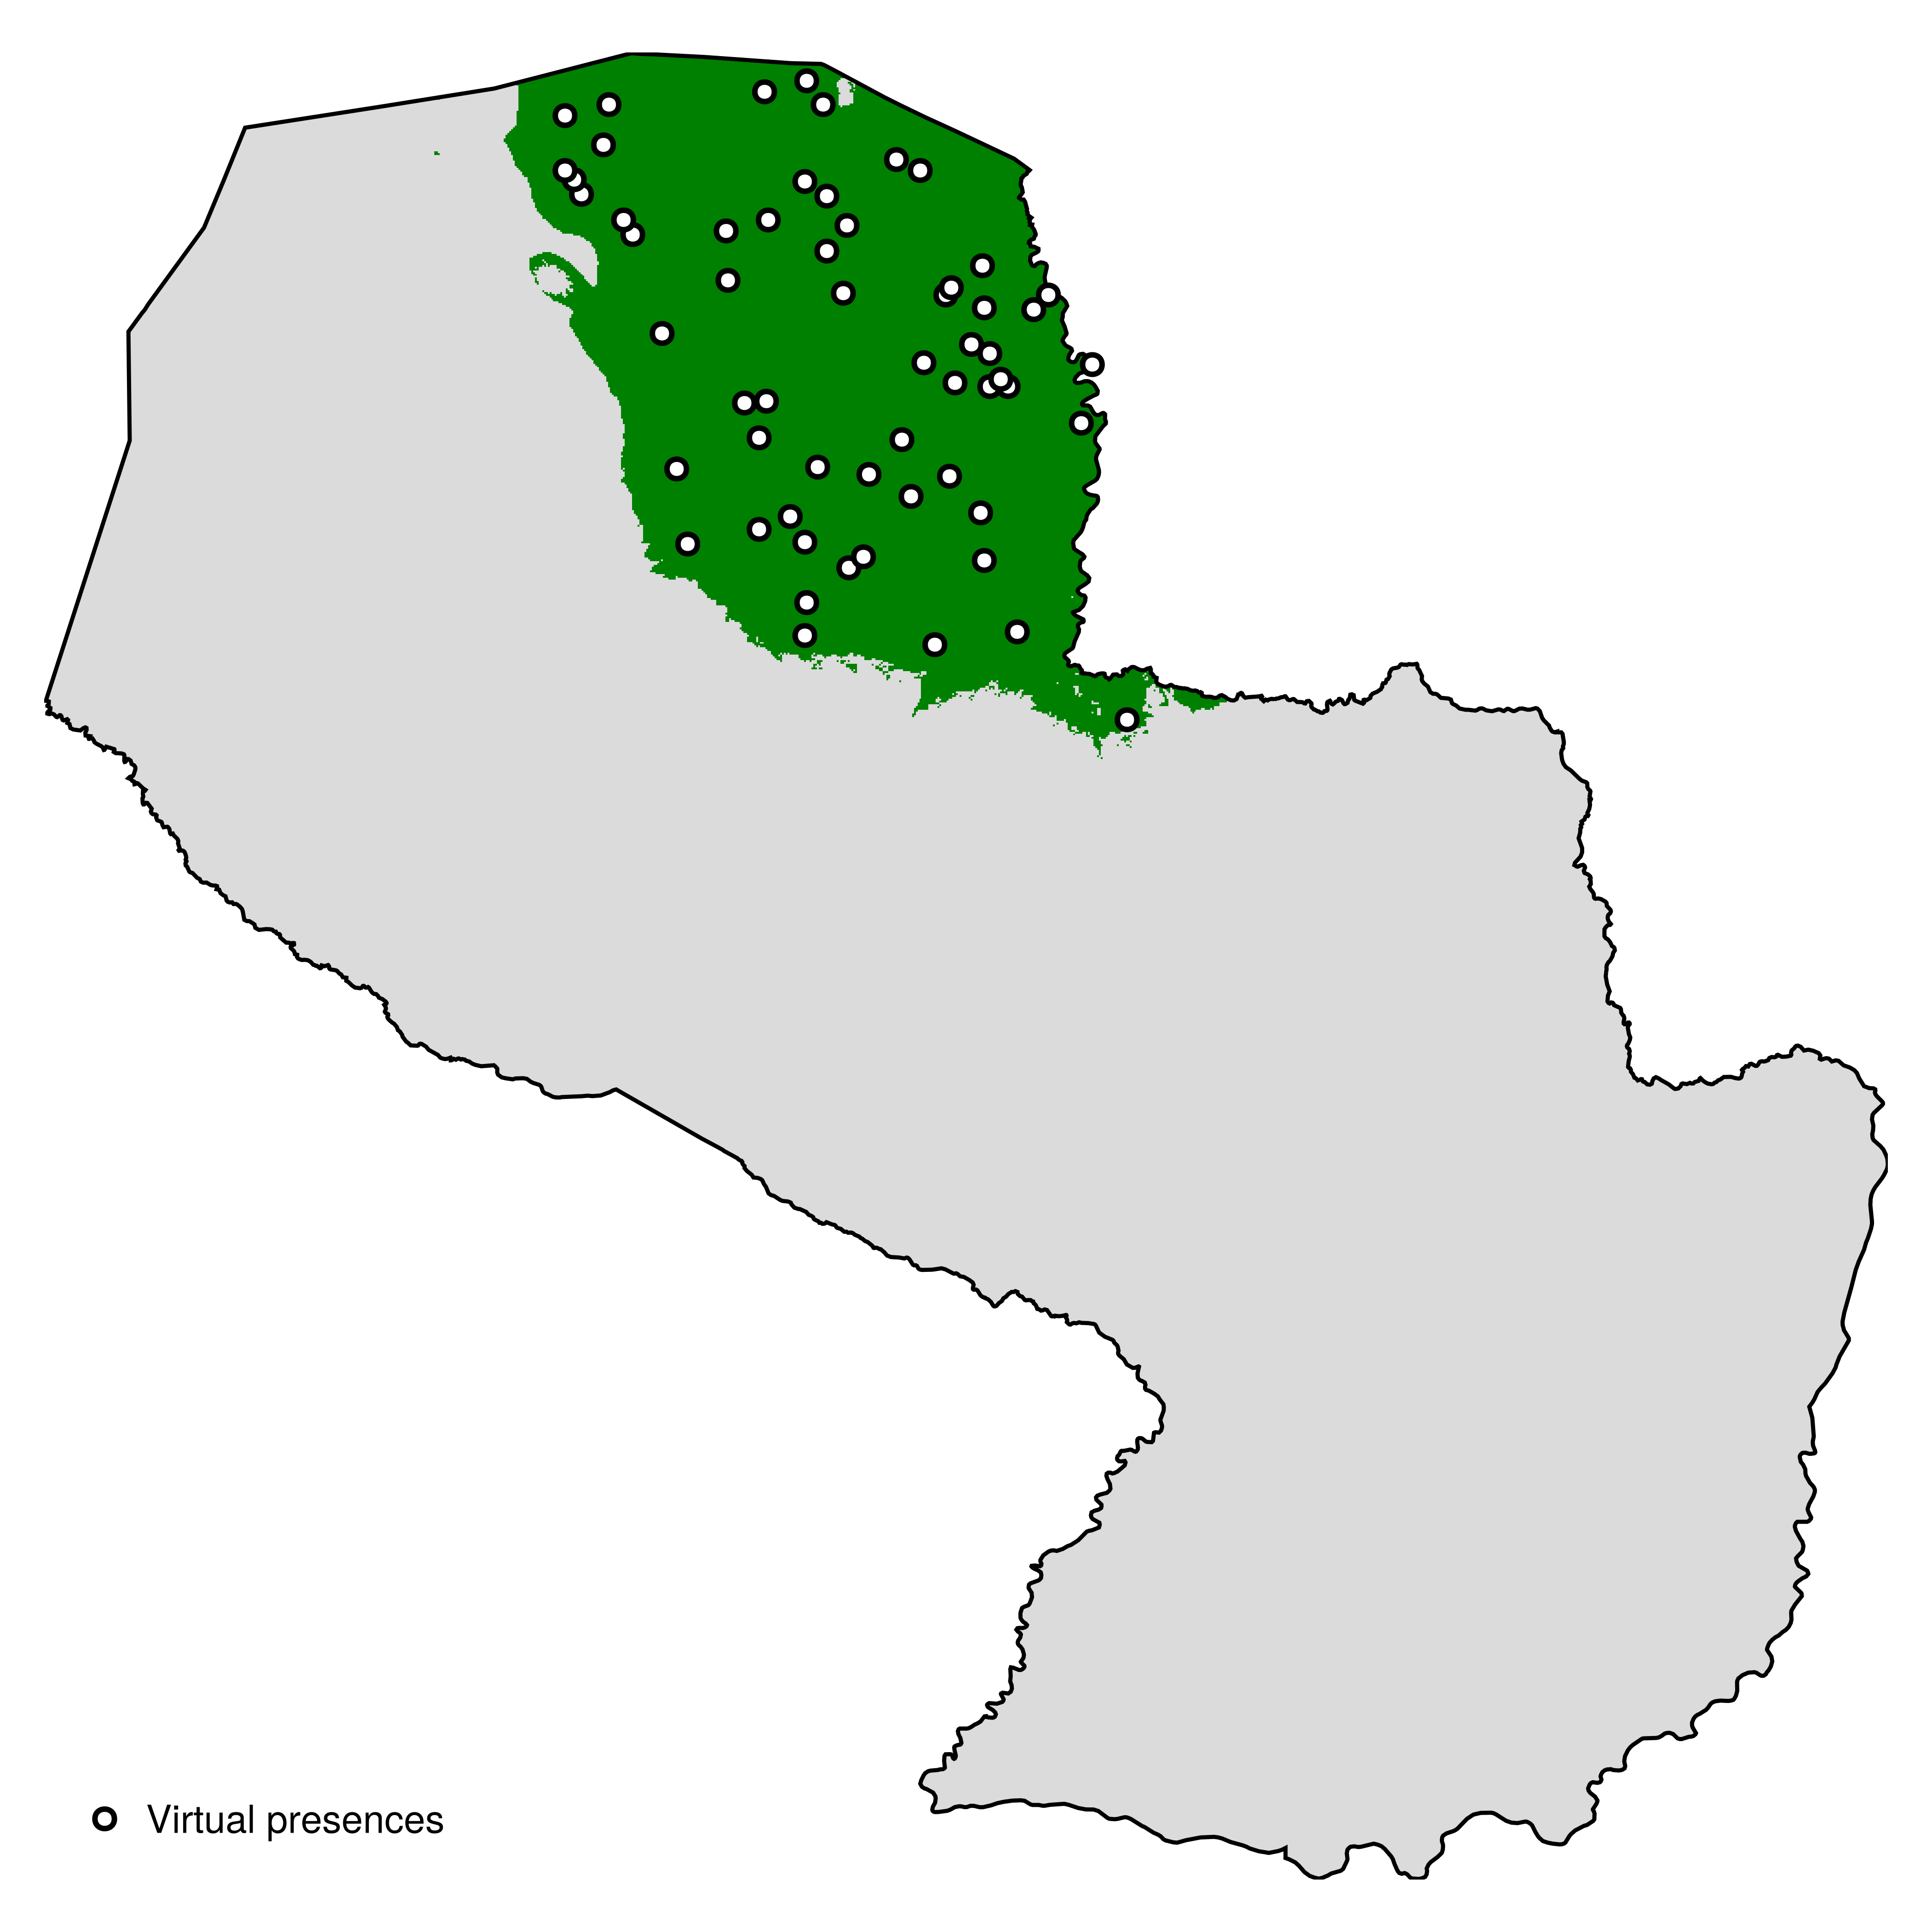
\includegraphics[keepaspectratio]{index_files/figure-latex/appendix-virtualspecies-fig-virtual-species-output-1.png}}

}

\caption{\label{fig-virtual-species}yeah}

\end{figure}%

\section*{References}\label{references}
\addcontentsline{toc}{section}{References}

\phantomsection\label{refs}
\begin{CSLReferences}{1}{0}
\bibitem[\citeproctext]{ref-Araujo2019}
Araújo, M. B., Anderson, R. P., Márcia Barbosa, A., Beale, C. M.,
Dormann, C. F., Early, R., Garcia, R. A., Guisan, A., Maiorano, L.,
Naimi, B., O'Hara, R. B., Zimmermann, N. E., \& Rahbek, C. (2019).
Standards for distribution models in biodiversity assessments.
\emph{Science Advances}, \emph{5}, eaat4858.
\url{https://doi.org/10.1126/sciadv.aat4858}

\bibitem[\citeproctext]{ref-Bagnall2018}
Bagnall, A., Flynn, M., Large, J., Line, J., Bostrom, A., \& Cawley, G.
(2018). Is rotation forest the best classifier for problems with
continuous features? \emph{arXiv {[}Cs.LG{]}}.

\bibitem[\citeproctext]{ref-Burgos2021}
Burgos, E. F., Vadell, M. V., Bellomo, C. M., Martinez, V. P., Salomon,
O. D., \& Gómez Villafañe, I. E. (2021). First evidence of akodon-borne
orthohantavirus in northeastern argentina. \emph{EcoHealth}, \emph{18},
429--439. \url{https://doi.org/10.1007/s10393-021-01564-6}

\bibitem[\citeproctext]{ref-Elith2009}
Elith, J., \& Leathwick, J. R. (2009). Species distribution models:
Ecological explanation and prediction across space and time.
\emph{Annual Review of Ecology, Evolution, and Systematics}, \emph{40},
677--697. \url{https://doi.org/10.1146/annurev.ecolsys.110308.120159}

\bibitem[\citeproctext]{ref-GBIF:TheGlobalBiodiversityInformationFacility2025}
GBIF: The Global Biodiversity Information Facility. (2025).
\emph{\emph{What is GBIF?}}

\bibitem[\citeproctext]{ref-Griffith2024}
Griffith, J., Lord, J.-M., Catchen, M. D., Arce-Plata, M. I., Bohorquez,
M. F. G., Chandramohan, M., Diaz-Corzo, M. C., Gravel, D., Gonzalez, L.
F. U., Gutiérrez, C., Helfenstein, I., Hoban, S., Kass, J. M., Laroque,
G., Laikre, L., Leigh, D., Leung, B., Mastretta-Yanes, A., Millette, K.,
\ldots{} Gonzalez, A. (2024). \emph{{BON} in a box: An open and
collaborative platform for biodiversity monitoring, indicator
calculation, and reporting}. \url{https://doi.org/10.32942/X2M320}

\bibitem[\citeproctext]{ref-Karger2017}
Karger, D. N., Conrad, O., Böhner, J., Kawohl, T., Kreft, H.,
Soria-Auza, R. W., Zimmermann, N. E., Linder, H. P., \& Kessler, M.
(2017). Climatologies at high resolution for the earth's land surface
areas. \emph{Scientific Data}, \emph{4}, 170122.
\url{https://doi.org/10.1038/sdata.2017.122}

\bibitem[\citeproctext]{ref-Kass2024-vy}
Kass, J. M., Smith, A. B., Warren, D. L., Vignali, S., Schmitt, S.,
Aiello-Lammens, M. E., Arlé, E., Márcia Barbosa, A., Broennimann, O.,
Cobos, M. E., Guéguen, M., Guisan, A., Merow, C., Naimi, B., Nobis, M.
P., Ondo, I., Osorio-Olvera, L., Owens, H. L., Pinilla-Buitrago, G. E.,
\ldots{} Zurell, D. (2024). Achieving higher standards in species
distribution modeling by leveraging the diversity of available software.
\emph{Ecography}. \url{https://doi.org/10.1111/ecog.07346}

\bibitem[\citeproctext]{ref-Kellner2025}
Kellner, K. F., Doser, J. W., \& Belant, J. L. (2025). Functional {R}
code is rare in species distribution and abundance papers.
\emph{Ecology}, \emph{106}, e4475.
\url{https://doi.org/10.1002/ecy.4475}

\bibitem[\citeproctext]{ref-Leroy2016}
Leroy, B., Meynard, C. N., Bellard, C., \& Courchamp, F. (2016).
Virtualspecies, an {R} package to generate virtual species
distributions. \emph{Ecography}, \emph{39}, 599--607.
\url{https://doi.org/10.1111/ecog.01388}

\bibitem[\citeproctext]{ref-Osborne2022}
Osborne, O. G., Fell, H. G., Atkins, H., Tol, J. van, Phillips, D.,
Herrera-Alsina, L., Mynard, P., Bocedi, G., Gubry-Rangin, C., Lancaster,
L. T., Creer, S., Nangoy, M., Fahri, F., Lupiyaningdyah, P., Sudiana, I.
M., Juliandi, B., Travis, J. M. J., Papadopulos, A. S. T., \& Algar, A.
C. (2022). Fauxcurrence: Simulating multi‐species occurrences for null
models in species distribution modelling and biogeography.
\emph{Ecography}, \emph{2022}, e05880.
\url{https://doi.org/10.1111/ecog.05880}

\bibitem[\citeproctext]{ref-Owen2010}
Owen, R. D., Goodin, D. G., Koch, D. E., Chu, Y.-K., \& Jonsson, C. B.
(2010). Spatiotemporal variation in akodon montensis (cricetidae:
Sigmodontinae) and hantaviral seroprevalence in a subtropical forest
ecosystem. \emph{Journal of Mammalogy}, \emph{91}, 467--481.
\url{https://doi.org/10.1644/09-MAMM-A-152.1}

\bibitem[\citeproctext]{ref-Tuanmu2014}
Tuanmu, M.-N., \& Jetz, W. (2014). A global 1‐km consensus land‐cover
product for biodiversity and ecosystem modelling: Consensus land cover.
\emph{Global Ecology and Biogeography: A Journal of Macroecology},
\emph{23}, 1031--1045. \url{https://doi.org/10.1111/geb.12182}

\bibitem[\citeproctext]{ref-Zurell2020}
Zurell, D., Franklin, J., König, C., Bouchet, P. J., Dormann, C. F.,
Elith, J., Fandos, G., Feng, X., Guillera-Arroita, G., Guisan, A.,
Lahoz-Monfort, J. J., Leitão, P. J., Park, D. S., Townsend Peterson, A.,
Rapacciuolo, G., Schmatz, D. R., Schröder, B., Serra-Diaz, J. M.,
Thuiller, W., \ldots{} Merow, C. (2020). A standard protocol for
reporting species distribution models. \emph{Ecography}, \emph{43},
1261--1277. \url{https://doi.org/10.1111/ecog.04960}

\end{CSLReferences}





\end{document}
